\section{Clonación de tarjetas SD para tarjetas Zybo}
\hypertarget{InstalacionLinux}{}
\subsection{Clonación de Linux en tarjeta SD}
Como sistema operativo de las tarjetas Zybo, usaremos el que creó nuestro compañero Gabriel Fernando Sánchez Reina \hyperlink{2}{[2]}, el cual ya está preparado para usar el IP hardware de Cristian Ambrosio Costoya \hyperlink{1}{[1]}.

Para ello, seguiremos los siguientes pasos:
\begin{itemize}
	\item Insertaremos la tarjeta SD con el sistema operativo en nuestro ordenador.
	\item Mediante la herramienta \texttt{dd} \hyperlink{5}{[5]}, guardaremos un fichero con extensión \texttt{.img} en nuestro ordenador, que será la copia de seguridad de la tarjeta SD.
	\begin{center}
		\texttt{sudo dd if=/dev/sdb of=/media/jesus/Gabri/Zybo.img}
	\end{center}
	\item A continuación, introducimos una tarjeta SD vacía de igual o mayor capacidad en nuestro ordenador.
	\item Mediante la herramienta \texttt{dd}, restauramos la copia de seguridad anterior en la nueva tarjeta SD.
	\begin{center}
		\texttt{sudo dd if=/media/jesus/Gabri/Zybo.img of=/dev/sdb}
	\end{center}
\end{itemize}

\subsection{Inicio de Linux desde la tarjeta SD}
Para iniciar la tarjeta con Linux debemos seguir los siguientes pasos:
\begin{itemize}
	\item Insertar la tarjeta SD en la placa Zybo.
	\item Cambiar el jumper JP5 a la posición SD para que arranque desde dicha tarjeta SD.
	\item Conectamos el cable USB de la placa al ordenador y arrancamos la placa.
	\item Abrimos un terminal PuTTY en la consola del ordenador\footnote{Puerto ttyUSB1 y velocidad 115200.} y ahora podemos ver como sí tenemos señal y arranca el sistema operativo.
\end{itemize}

\newpage
\subsection{Creación de usuarios}
Al ser la primera vez que arrancamos el sistema operativo Linux, contamos únicamente con el usuario \texttt{root}, cuya contraseña es \texttt{root}. Por lo tanto, tenemos que crear otro usuario, que será con el que iniciemos sesión en las placas usando el comando:
\begin{center}
	\texttt{adduser zyboX}
\end{center}
Donde \texttt{X} es el identificador de la placa con la que estamos trabajando.

A continuación, tendremos que rellenar los siguientes campos:
\begin{itemize}
	\item \textbf{Contraseña de usuario:} Introducimos la contraseña para el usuario creado. Si seguimos la nomenclatura que sigue el proyecto, será \texttt{zyboX}.
	\item \textbf{Repetir contraseña:} Repetiremos la contraseña para comprobar que no nos hemos equivocado.
	\item \textbf{Nombre:} Pondremos el nombre del usuario, \texttt{zyboX}, siguiendo la nomenclatura del proyecto.
	\item \textbf{Número de habitación, teléfono de trabajo y de casa, y ``otro'':} Presionamos la tecla \texttt{ENTER} para dejarlo por defecto y continuar.
\end{itemize}

\begin{figure}[h]
	\centering
	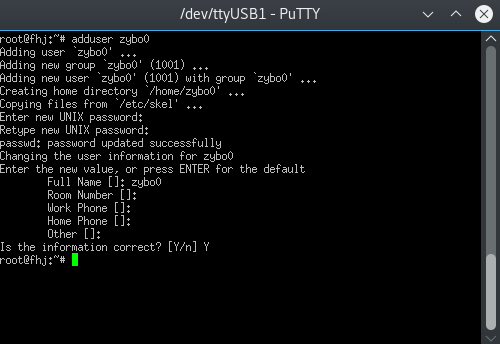
\includegraphics[scale=0.9]{Anexos/Anexo2/Linux/NuevoUsuario.png}
	\caption{Ejemplo de creación del usuario zybo0}
	\label{Ejemplo de creación del usuario zybo0}
\end{figure}


\subsection{Habilitar SSH en placas Zybo}
Para establecer una conexión entre el ordenador central y las placas, tendremos que usar el protocolo SSH, que viene deshabilitado por defecto en Linux.

Para habilitarlo tendremos que acceder al archivo \texttt{/etc/ssh/sshd\_config} como super-usuario. Para ello, utilizaremos el siguiente comando:
\begin{center}
	\texttt{nano /etc/ssh/sshd\_config}
\end{center}
A continuación, nos dirigimos a la línea que tiene la siguiente sentencia:
\begin{center}
	\texttt{\#PasswordAuthentification yes}
\end{center}
Borramos la almohadilla (\#), guardamos y cerramos el fichero.
\begin{figure}[h]
	\centering
	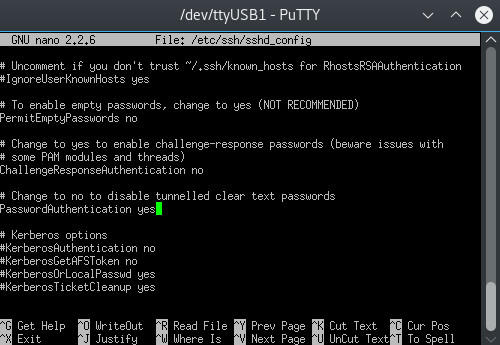
\includegraphics[scale=0.8]{Anexos/Anexo2/Linux/SSH.png}
	\caption{Fichero \texttt{sshd\_config} modificado}
	\label{Fichero ssh_d modificado}
\end{figure}

\newpage
Para establecer los cambios realizados, debemos reiniciar el servicio SSH. Para ello utilizamos:
\begin{center}
	\texttt{/etc/init.d/ssh restart}
\end{center}
\begin{figure}[h]
	\centering
	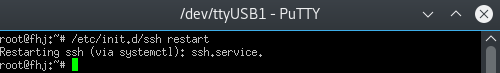
\includegraphics[scale=0.8]{Anexos/Anexo2/Linux/SSHRestart.png}
	\caption{Reiniciando el servicio SSH}
	\label{Reiniciando el servicio SSH}
\end{figure}

A partir de aquí ya podemos establecer conexiones SSH desde el ordenador central al resto de placas Zybo y enviar cualquier tipo de ficheros bien sea desde el ordenador central a las placas o bien, entre placas.